%%% LaTeX Template: Two column article
%%%
%%% Source: http://www.howtotex.com/
%%% Feel free to distribute this template, but please keep to referal to http://www.howtotex.com/ here.
%%% Date: February 2011

%%% Preamble
\documentclass[	
	DIV=calc,
	paper=a4,
	fontsize=11pt,
	onecolumn
]{scrartcl} % KOMA-article class

\usepackage{lipsum} % Package to create dummy text
\usepackage{float}
\usepackage[utf8x]{inputenc}
\usepackage[italian]{babel} % English language/hyphenation
\usepackage[protrusion=true,expansion=true]{microtype} % Better typography
\usepackage{amsmath,amsfonts,amsthm} % Math packages
\usepackage[pdftex]{graphicx} % Enable pdflatex
\usepackage[svgnames]{xcolor} % Enabling colors by their 'svgnames'
\usepackage[hang, small,labelfont=bf,up,textfont=it,up]{caption} % Custom captions under/above floats
\usepackage{epstopdf} % Converts .eps to .pdf
\usepackage{subfig} % Subfigures
\usepackage{booktabs} % Nicer tables
\usepackage{fix-cm} % Custom fontsizes

%%% Custom sectioning (sectsty package)
\usepackage{sectsty} % Custom sectioning (see below)
\allsectionsfont{ % Change font of al section commands
	\usefont{OT1}{}{b}{n} % bch-b-n: CharterBT-Bold font
}

\sectionfont{ % Change font of \section command
	\usefont{OT1}{}{b}{n} % bch-b-n: CharterBT-Bold font
}

%%% Headers and footers
\usepackage{fancyhdr}												% Needed to define custom headers/footers
	\pagestyle{fancy}														% Enabling the custom headers/footers
\usepackage{lastpage}	

% Header (empty)
\lhead{}
\chead{}
\rhead{}
% Footer (you may change this to your own needs)
\lfoot{
	\footnotesize 
	\texttt{Andrea Aquino, Michele Consiglio. DHT Symphony Simulation} 
}
\cfoot{}
\rfoot{
	\footnotesize 
	pagina 
	\thepage\ 
	di 
	\pageref{LastPage}
}
\renewcommand{\headrulewidth}{0.0pt}
\renewcommand{\footrulewidth}{0.4pt}

%%% Creating an initial of the very first character of the content
\usepackage{lettrine}
\newcommand{\initial}[1]{
	\lettrine[lines=3,lhang=0.3,nindent=0em]{
     \color{Black}
     {\textsf{#1}}}{}}

%%% Title, author and date metadata
\usepackage{titling}															% For custom titles

\newcommand{\HorRule}{\color{DarkRed} % Creating a horizontal rule
\rule{\linewidth}{1pt}
}

\pretitle{
	\vspace{-60pt} 
	\begin{flushleft} 
		\HorRule 
		\fontsize{40}{50} 
		\usefont{OT1}{}{b}{n} 
		\color{DarkRed} 
		\selectfont 
}
	
	\title{DHT Symphony Simulation}					% Title of your article goes here
	\posttitle{
		\par
	\end{flushleft}
		\vskip 0.5em
	}

\preauthor{
	\begin{flushleft}
		\large 
		\lineskip 0.5em 
		\usefont{OT1}{}{b}{sl} 
		\color{DarkRed}
}
\author{Andrea Aquino, Michele Consiglio}											% Author name goes here
\postauthor{
	\footnotesize 
	\usefont{OT1}{}{m}{sl} 
	\color{Black} 
	Università di Bologna 								% Institution of author
	\par
	\end{flushleft}
	\HorRule
}

\date{\today}																				% No date

%%% Begin document
\begin{document}
	\maketitle
	\thispagestyle{fancy} % Enabling the custom headers/footers for the first page 
	\begin{abstract}
	Il protocollo DHT Symphony discusso da Manku, Bawa e Raghavan si propone come nuova frontiera per il mantenimento e l'accesso di dizionari distribuiti sulla rete globale. Sfruttando una topologia di rete virtuale ad anello sulla quale vengono instaurate connessioni tra nodi distanti, è possibile ridurre drasticamente i tempi di recupero di dati evitandone l'eccessiva replicazione. Tuttavia il numero di messaggi necessari al funzionamento del protocollo stesso non è oggetto di studio del documento prodotto dagli autori di cui sopra. Si intende quindi analizzare tale aspetto mediante la simulazione del protocollo a mezzo del simulatore Omnet++. Verrà inoltre introdotta una modifica protocollare con lo scopo di diminuire il numero di messaggi transitanti nella rete senza inficiare la correttezza e l'efficacia del protocollo.
	\end{abstract}
	
\section{Protocollo DHT Symphony}
	Al fine di realizzare una tabella hash distribuita affidabile è necessario che si mantengano copie dei dati in essa contenuti su svariate macchine facenti parte della rete che compone la tabella stessa. In pratica ciò è quasi sempre inattuabile. Il protocollo DHT Symphony tenta di risolvere il problema eleggendo dei candidati facenti parte della rete per la gestione e la memorizzazione di determinate porzioni della tabella. Affinché l'accesso ai dati in essa contenuti sia efficiente i nodi vengono organizzati in una struttura circolare in modo che ogni nodo abbia un vicino ad esso immediatamente precedente ed uno successivo. Questo approccio garantisce la raggiungibilità di qualsiasi macchina della DHT a partire da qualunque altra in un numero di passi non maggiore della metà del numero di nodi facenti parte della rete. Al fine di ridurre ulteriormente questo valore il protocollo introduce delle connessioni ulteriori tra nodi non adiacenti instaurate a mezzo di una particolare distribuzione di probabilità (distribuzione armonica da cui il protocollo trae il suo nome). Per poter comprendere al meglio il suo funzionamento è consigliabile pensare alla totalità dei dati contenuti nella DHT come se fossero posti su una circonferenza di perimetro unitario. Ogni nodo facente parte della rete occupa una posizione differente su tale circonferenza e si occupa di soddisfare le richieste (in gergo, \textit{fa da manager}) per la porzione di dati contenuta tra il nodo medesimo ed il suo immediato vicino in senso antiorario. Si noti che:
\begin{itemize}
	\item[1.] Sebbene un nodo sia connesso ai due nodi a lui adiacenti e a svariati altri non conosce il punto preciso che questi occupano sulla circonferenza. Tale informazione è di vitale importanza per il funzionamento di diversi punti del protocollo;
	\item[2.] Inoltre essendo la rete particolarmente dinamica, il protocollo gestisce l'accesso e l'uscita di nodi in modo che i dati della DHT rimangano consistenti. In particolare quando un nodo intende accedere alla rete decide autonomamente in quale punto della circonferenza posizionarsi mediante la scelta randomica di un valore uniformemente distribuito nell'intervallo [0,1). Informa poi un nodo già connesso della sua volontà di accedere alla rete distribuita; mediante un protocollo di instradamento interno noto come \textit{protocollo di routing} tale nodo contatta l'attuale manager di quel punto permettendo al nuovo nodo di accedere previa modifica delle connessioni opportune.
\end{itemize}
Il protocollo consta di tutta una serie di sottoprotocolli più o meno complessi che gli permettono di operare nella sua interezza. Per informazioni più dettagliate si rimanda il lettore al documento ``DHT Symphony: Distributed hashing in a small world''[1.]

\section{Simulazione}
	\subsection{Gli strumenti}
	Lo studio di simulazione è stato realizzato a mezzo del simulatore Omnet++. Nello specifico il protocollo oggetto dello studio è stato emulato mediante l'implementazione dei moduli stanti alla lista seguente:
	\begin{itemize}
		\item File NED descrivente la topologia di rete virtuale;
		\item Classe rappresentante i singoli nodi all'interno della rete;
		\item Pacchetti di rete strutturati per la trasmissione delle informazioni protocollari rilevanti;
		\item File di configurazione per gestire le informazioni parametriche della simulazione.
	\end{itemize}
	Sono stati inoltre utilizzati gli strumenti di analisi offline messi a disposizione da tale simulatore per l'analisi prestazionale del protocollo nella versione originale e soggetto a modifica. I risultati di tale studio verranno discussi nella sezione ``Risultati'' del presente elaborato.
	\subsection{Il livello di dettaglio}
	L'implementazione in esame consiste a tutti gli effetti in una emulazione puntuale del protocollo DHT Symphony allo scopo di analizzare con assoluta precisione le prestazioni dello stesso in termini di numero di messaggi scambiati tra i nodi della rete al passare del tempo. La simulazione di rete astrae dalla topologia di rete reale realizzando soltanto le connessioni virtuali previste dal protocollo medesimo. In particolare i nodi sono disposti su di un ipotetico cerchio di perimetro unitario che costituisce una rete ad anello. Nella fase di inizializzazione del protocollo ogni nodo è quindi connesso ai suoi due immediati vicini ed è dotato di un numero K (configurabile) di connessioni ``lunghe'' con i nodi i cui id differiscono dal proprio tra le 8 e le 8+K unità. \\*\\*
Per semplicità le connessioni con i nodi vicini (da qui in poi connessioni brevi) sono state realizzate mediante gate bidirezionali facenti parte di un vettore di gate contenente la totalità delle connessioni per il nodo corrente. In fase di sperimentazione il numero di nodi della rete è stato fissato a 16, 32 e 64, di cui la metà connessi nella struttura ad anello discussa in precedenza e la rimanente metà in principio non connessa.\\*\\* 
Infine sono stati individuati e simulati fedelmente i seguenti aspetti del protocollo:
	\begin{itemize}
		\item[1.] stima della lunghezza del segmento gestito da un nodo;
		\item[2.] stima del numero di nodi della rete;
		\item[3.] protocollo di routing per individuare il manager di un punto qualsiasi sull'anello di perimetro unitario;
		\item[4.] protocollo di relink;
		\item[5.] protocollo di join;
		%\item[6.] protocollo di leave.		
	\end{itemize}

\begin{figure}[H]
	\centering
	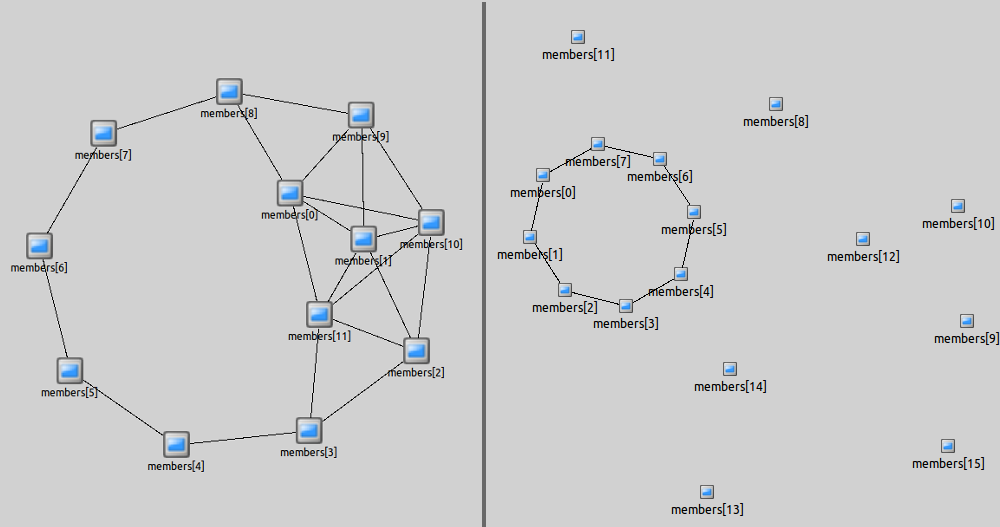
\includegraphics[scale=0.35]{topologia.png}
	\caption{Topologie di reti virtuali}
	\label{Figura 1}
\end{figure}

	\subsection{Assunzioni}
	Il documento ``Symphony: Distributed Hashing In A Small World'' non specifica una variegata serie di dettagli. Pertanto è stato necessario effettuare tutta una serie di assunzioni al fine di poter implementare il protocollo stesso.
	\begin{itemize}
	\item[1.] La rete è supposta essere, in principio, popolata;
	\item[2.] Il numero di nodi della DHT è inferiormente limitato da un valore positivo configurabile, supposto maggiore di 8;
	\item[3.] Ogni nodo non ha accesso diretto al valore indicante la posizione all'interno della circonferenza di perimetro unitario dei propri vicini, deve pertanto recuperarla chiedendola esplicitamente a questi mediante l'uso di messaggi di rete. Il protocollo Symphony assume che la posizione dei nodi manager del segmento immediatamente precedente e del segmento immediatamente successivo di un dato nodo sia direttamente accessibile in ogni momento. Ciò ha perfettamente senso in termini matematici in quanto ogni nodo altro non è che una particolare struttura dotata di collegamenti ai nodi vicini. Tuttavia i nodi descritti dal protocollo sono a tutti gli effetti macchine connesse attraverso la rete, ne deriva il non trascurabile dettaglio implementativo che consiste nel dover recuperare tali valori a mezzo messaggi mediati dai canali di comunicazione dai nodi adiacenti. 
	\item[4.] Il lookup dei file della DHT non è ritenuto di interesse e pertanto non è simulato;
	\item[5.] Nessuna coppia di nodi facente parte della DHT ha la stessa posizione sulla circonferenza di perimetro unitario. In linea teorica pescando valori randomici dalla distribuzione armonica del protocollo in esame due nodi diversi potrebbero ottenere lo stesso valore. Ciò significherebbe che entrambi i nodi sono manager della stessa porzione della DHT. Il protocollo Symphony non dichiara come affrontare questo particolare problema, che crea ambiguità in fase di esecuzione del sottoprotocollo di join.
	\end{itemize}
	
\section{Modifica protocollare}
	L'implementazione originale del protocollo di routing prevede, in virtù del punto 3. della sezione ``Assunzioni'', la necessità di effettuare un broadcast ai nodi vicini per poter definire quali di questi dista meno dal nodo destinazione e quindi instradare le successive richieste attraverso di esso. In fase di simulazione suddetto dettaglio sembra inficiare duramente la qualità del protocollo in termini prestazionali (quantità di messaggi trasmessi). Quindi, sotto l'assunzione che ogni nodo mantenga traccia della posizione dei suoi vicini sulla circonferenza di perimetro unitario, è stata effettuata una modifica protocollare che snellisce sostanzialmente il protocollo di routing (massivamente sfruttato anche da parte dei protocolli di join e di relink) sotto tale punto di vista. 	
	\subsection{Implementazione}	
	In teoria sarebbe stato necessario tenere traccia per ogni nodo della posizione di ogni altro nodo ad esso connesso mediante un vettore locale. Si noti che la posizione dei vicini di un dato nodo può variare solamente a seguito dell'accesso o dell'uscita di un nodo dalla rete; si ritiene che tale evento occorra assai più raramente rispetto al protocollo di routing (che è cuore del meccanismo di inserimento e ricerca di chiavi nel dizionario distribuito). Per semplicità, tale vettore è stato assunto esistere e la posizione dei nodi vicini al nodo corrente è stata recuperata mediante le direttive del simulatore Omnet++ stesso. 
	\subsection{Correttezza}
	La modifica protocollare precedentemente discussa non modifica in alcun modo la semantica del protocollo. Segue una dimostrazione informale di tale evidenza:
\begin{itemize}
	\item[1.] la modifica in esame riguarda esclusivamente il protocollo di routing; se la semantica di tale protocollo rimane la medesima, di conseguenza la semantica del protocollo complessivo non varia.
	\item[2.] per dimostrare che la semantica del protocollo di routing non cambia è sufficiente dimostrare che in ogni caso in cui la versione originale del protocollo effettua una scelta tra i nodi vicini per l'instradamento di una richiesta, il protocollo modificato effettua la medesima scelta.
	\item[3.] dimostriamo il punto 2. per induzione sul numero di connessioni lunghe del nodo corrente. 
	\begin{itemize}
	\item \textbf{caso base}: il nodo corrente ha solo le connessioni brevi con i nodi che lo seguono immediatamente in senso orario e antiorario. Poiché sono supposti esistere almeno 3 nodi all'interno della rete simulata, deve esistere una relazione d'ordine totale tra le posizioni di questi sulla circonferenza di perimetro unitario. Siano \[0 \leq a \neq b \neq c < 1\] tali posizioni e sia \[0 \leq x < 1\] il valore di cui si intende individuare il nodo manager per mezzo del protocollo di routing. Ne consegue che \[|a-x| \neq |b-x| \neq |c-x|\] e quindi una sola distanza è quella minima. Non essendoci alcuna forma di non determinismo ed essendo la stima di a, b e c uguale per entrambe le versioni del protocollo la scelta di instradamento non subisce variazioni.
	\item \textbf{caso induttivo}: supponiamo che i protocolli si comportino allo stesso modo per un certo numero n di link lunghi. Dimostriamo che continuano a comportarsi allo stesso modo anche per n+1 link lunghi. In virtù del punto 5. della sezione ``Assunzioni'' il nodo connesso al nodo corrente mediante l'n+1-esimo link lungo ha una posizione diversa da tutti gli altri sulla circonferenza di perimetro unitario. I casi sono dunque due:
		\begin{itemize}
			\item il nuovo nodo è il più vicino al nodo destinazione; ma in tal caso lo è per entrambe le versioni del protocollo e quindi i protocolli continuano ad instradare i messaggi mediante lo stesso nodo.
			\item il nuovo nodo è più distante rispetto ad un altro vicino del nodo corrente dal nodo destinazione; ma in tal caso il protocollo si comporta come nel caso in cui l'n+1-esimo link lungo non esista affatto, ma in questa situazione i due protocolli hanno lo stesso comportamento \underline{per ipotesi induttiva}.
		\end{itemize}
	\end{itemize} 
\end{itemize}
Fino ad ora abbiamo supposto che la posizione dei nodi vicini al nodo che sta correntemente eseguendo il protocollo di routing sia costantemente aggiornata per la versione modificata del protocollo. Ciò è tuttavia certamente vero sotto l'ipotesi che nel momento in cui un nodo accede alla rete o immediatamente prima di abbandonarla comunichi ai propri vicini la necessità di aggiornare le posizioni dei nodi adiacenti.
\section{Risultati}


\begin{figure}[H]
	\centering
	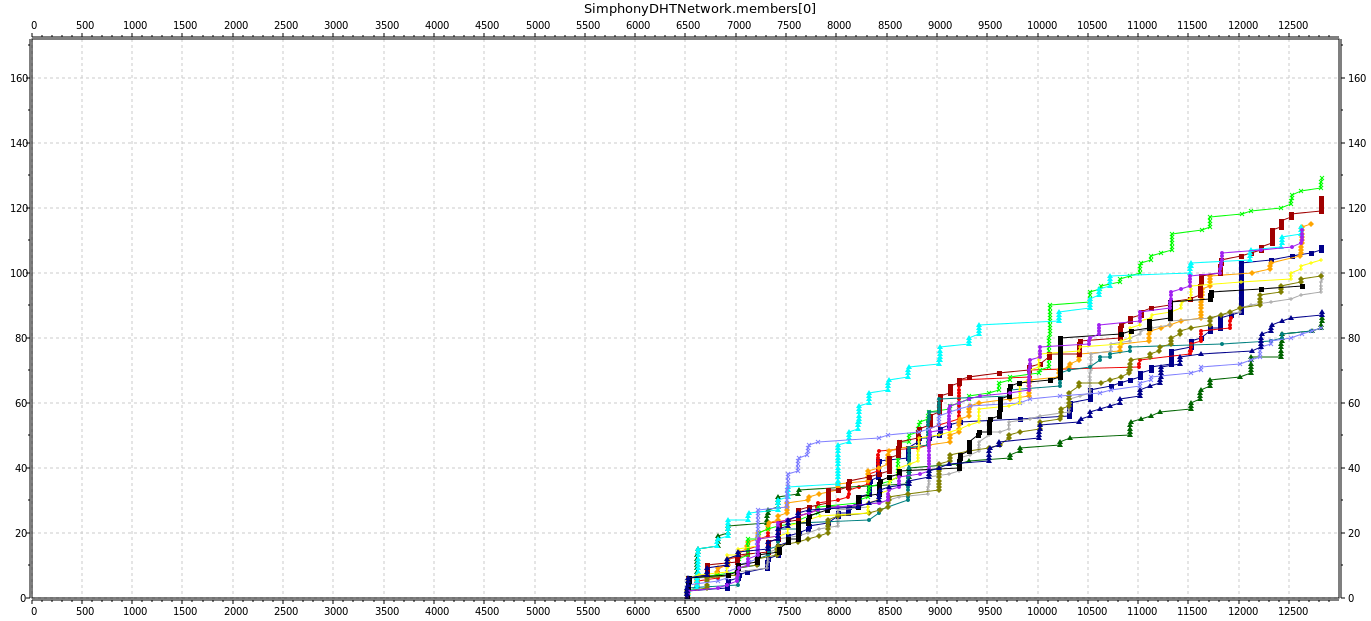
\includegraphics[scale=0.35]{SymphonyDHTMod/plots/MessagesSentByEveryNode/128_Nodes_FastAccess/SymphonyDHTMod_128Nodes_FastAccess_Node0.png}
	\caption{Topologie di reti virtuali}
	\label{Figura 1}
\end{figure}



\section{Bibliografia}
\begin{itemize}
\item[1.] Gurmeet Singh Manku, Mayank Bawa, and Prabhakar Raghavan. 2003. Symphony: distributed
hashing in a small world. In Proceedings of the 4th conference on USENIX Symposium on
Internet Technologies and Systems - Volume 4 (USITS'03), Vol. 4. USENIX Association,
Berkeley, CA, USA, 10-10
\item[2.] Omnet++ Network Simulation Framework - http://www.omnetpp.org/ 
\end{itemize}

\end{document}